\chapter{اتحاد و جستجوی اثبات}

\section{اتحاد}
در فصل قبل، هنگام کار روی KB4 با اتحاد یا unification آشنا شدیم. به عنوان مثال گفتیم که پرولوگ \متن‌لاتین{woman(X)} را با \متن‌لاتین{woman(mia)} متحد کرده و بنابراین متغیر X مقدار mia را به خود می‌گیرد. حال می‌خواهیم کمی دقیقتر به unification‌ نگاه کنیم.

به خاطر دارید که در پرولوگ سه نوع ترم داشتیم:

\begin{enumerate}
\item ثوابت. شامل اتم‌ها مثل vincent و اعداد مثل 123
\item متغیرها. مثل X یا Z3
\item ترم‌های مرکب. به شکل \متن‌لاتین{functor(term\_1,...,term\_2)}
\end{enumerate}

در ادامه این فصل می‌خواهیم به تعریفی برسیم که پرولوگ بر اساس آن دو ترم را متحد می‌کند. برای شروع تعریف زیر را مطرح می‌کنیم. هرچند که این تعریف جامع نیست اما ایده اصلی را مشخص می‌کند.

دو ترم متحد می‌شوند اگر هر دو ترم، یکسان باشند یا شامل متغیرهایی باشند که بتوان آنها را طوری مقداردهی کرد که در نتیجه دو ترم یکسان شوند.

طبق این تعریف، به عنوان مثال، دو ترم mia و mia متحد می‌شوند زیرا هر دو اتم‌های یکسانی هستند. به طور مشابه 42 و 42 نیز متحد می‌شوند چون هر دو اعداد یکسانی هستند. دو ترم X و X هم به همین نحو متحد می‌شوند چون هر دو متغیر یکسان هستند و به همین ترتیب ترم‌های پیچیده \متن‌لاتین{woman(mia)} و \متن‌لاتین{woman(mia)} نیز. اما دو ترم مرکب \متن‌لاتین{woman(mia)} و \متن‌لاتین{woman(vincent)} متحد نمی‌شوند دو ترم یکسان نیستند و از متغیری هم ندارند که با مقداردهی آن بتوان دو ترم یکسان ساخت.

در مورد دو ترم X و mia وضعیت به چه ترتیب است؟ این دو ترم یکسان نیستند. ولی X یک متغیر است که می‌تواند مقدار بگیرد و اگر آن مقدار را برابر mia در نظر بگیریم، دو ترم یکسان خواهیم داشت. پس با استفاده از قسمت دوم تعریف بالا، دو ترم X و mia متحد می‌شوند. به همین نحو دو ترم \متن‌لاتین{woman(mia)} و \متن{woman(X)} متحد می‌شوند. در مورد \متن‌لاتین{loves(vincent,X)} و \متن‌لاتین{loves(X,mia)}، آیا اتحاد انجام می‌شود؟ مشخص است که به هیچ وجه ممکن نیست مقداری برای X بیابیم که این دو ترم یکسان شوند پس پاسخ منفی است.

معمولاً بیش از اینکه بخواهیم بدانیم آیا امکان اتحاد وجود دارد یا خیر، جالب است که بدانیم چطور متغیرها را مقداردهی کنیم تا دو ترم یکسان داشته باشیم. پرولوگ ابزاری است که این اطلاعات را در اختیار ما قرار می‌دهد. وقتی پرولوگ دو ترم را متحد می‌کند تمام مقداردهی‌های لازم برای یکسان سازی دو ترم را انجام می‌دهد. این حقیقت بعلاوه اینکه پرولوگ اجازه ایجاد ساخت‌های پیچیده و تودرتو را به ما می‌دهد، ابزار قدرتمندی برای برنامه‌نویسی در اختیارمان می‌گذارد.

حال که ایده اصلی را می‌دانیم، در زیر تعریف دقیقتری ارائه می‌دهیم. این تعریف نه‌تنها می‌گوید کدام ترم‌ها توسط پرولوگ قابل اتحاد هستند بلکه نحوه مقداردهی متغیرها برای نیل به این مقصود را نیز مشخص می‌کند.

\شروع{شمارش}
\فقره اگر term1 و term2 از ثوابت باشند، آنگاه این دو ترم متحد می‌شوند اگر و تنها اگر اتم‌های یکسان یا اعداد یکسان باشند.
\فقره اگر item1 یک متغیر باشد و item2 ترمی از هر نوع باشد، آنگاه این‌دو متحد می‌شوند و term1 به term2 مقداردهی خواهد شد. بطور مشابه اگر term2 یک متغیر باشد و term1 ترمی از هر نوع باشد، این‌دو متحد می‌شوند و term2 به term1 مقداردهی خواهد شد. (بنابراین اگر هر دو متغیر باشند، هردو به دیگری مقداردهی خواهند شد و می‌گوییم آنها مقدار اشتراکی دارند.)
\فقره اگر term1 و term2 ترم‌های مرکب باشند، آنگاه این‌دو ترم متحد می‌شوند اگر و تنها اگر:
\شروع{شمارش}
\فقره functor و arity یکسان داشته باشند، و
\فقره تمام آرگومان‌های آنها به ترتیب متحد شوند، و
\فقره مقداردهی متغیرها سازگار باشند. (برای مثال، اگر برای متحد کردن دو آرگومان اول مقدار X برابر mia قرار داده‌شد، نمی‌توان برای متحد کردن آرگومان‌های بعدی X را با vincent مقداردهی کرد.)
\پایان{شمارش}
\فقره دو ترم متحد می‌شوند اگر و تنها اگر از اعمال سه بند بالا نتیجه شود که آنها قابل اتحاد هستند.
\پایان{شمارش}

اولین بند تعریف بالا، شرایط unify‌ شدن دو ثابت را نشان می‌دهد. دومین بند شرایط unify شدن یک متغیر و یک ترم را تعریف می‌کند و می‌گوید چطور مقداردهی را انجام دهیم تا دو ترم یکسان شوند. در آخر، بند سوم مشخص می‌کند که دو ترم مرکب چطور متحد می‌شوند. بند چهارم از تعریف بالا نیز مهم است. این بند می‌گوید که سه بند اول تمام چیزی است که برای اتحاد ترم‌ها نیاز داریم. اگر دو ترم در هیچ‌یک از سه بند جای نگیرند، هیچگاه قابل اتحاد نخواهند بود. ترم batman و \متن‌لاتین{ daughter(ink)} را در نظر بگیرید. اولی یک ثابت است و دومی یک ترم مرکب. هیچکدام از سه بند اول در مورد اتحاد این دو نوع صحبت نمی‌کنند. لذا طبق بند چهارم این دو ترم قابل اتحاد نیستند.

\subsection{مثال‌ها}
برای اینکه از تفهیم تعریف بالا مطمئن باشیم، بیایید چند مثال را با هم ببینیم. در این مثال‌ها از محمول از پیش تعریف شده \متن‌لاتین{=/2} استفاده می‌کنیم.(به خاطر بیاورید که \متن‌لاتین{/2} نشان‌دهنده این است که محمول دو آرگومان می‌گیرد.) این محمول چک می‌کند که آیا دو آرگومانش قابل اتحاد هستند یا خیر. به مثال زیر توجه کنید.

\begin{latin}
\begin{lstlisting}
?- =(mia,mia).
true.
?- =(mia,vincent).
false.
\end{lstlisting}
\end{latin}

البته معمولاً از محمول \متن‌لاتین{=/2} به صورتی که دیدید استفاده نمی‌کنیم. پرولوگ به ما اجازه می‌دهد که functor  \متن‌لاتین{=/2} را بین دو آرگومان قرار دهیم:

\begin{latin}
\begin{lstlisting}
?- mia = mia.
true.
?- 2 = 2.
true.
?- mia = vincent.
false.
\end{lstlisting}
\end{latin}

اما چرا پرسش \متن‌لاتین{mia = mia} با پاسخ مثبت همراه بود؟ اگرچه واضح است اما بهتر است ببینیم چطور از تعریف بالا به این نتیجه می‌رسیم.

تعریف سه بند دارد که بند دوم مربوط به حالتی است که یکی از دو ترم متغیر باشند، و بند سوم نیز برای حالتی است که هر دو ترم، مرکب باشند، ولی در مثال ما اینچنین نیست. ولی بند اول مربوط به مثال ماست. در این بند گفته می‌شود که دو ترم ثابت متحد می‌شوند اگر و تنها اگر هر دو یکسان باشند. چون mia و mia اتم‌های یکسانی هستند پس اتحاد صورت می‌گیرد. همین استدلال برای 2 و 2 برقرار است. در مورد mia و vincent هر دو اتم هستند ولی یکسان نیستند پس پرولوگ پاسخ منفی داده‌است.

بیایید مثال دیگری را بررسی کنیم:

\begin{latin}
\begin{lstlisting}
?- 'mia' = mia.
true.
\end{lstlisting}
\end{latin}

چرا این دو ترم متحد شدند؟  برای پرولوگ \متن‌لاتین{'mia'} و \متن‌لاتین{mia} دو ترم یکسان هستند. در واقع برای پرولوگ، هر اتمی به شکل \متن‌لاتین{'symbol'} با اتمی به شکل \متن‌لاتین{symbol} یکسان است. اما

\begin{latin}
\begin{lstlisting}
?- '2' = 2.
false.
\end{lstlisting}
\end{latin}

پرولوگ پاسخ منفی داد. اگر کمی به تعاریف فصل یک دقت کنید متوجه می‌شوید که 2 یک عدد است ولی '2' یک اتم است. طبیعی است که این دو یکسان نیستند و نمی‌توانند متحد شوند.

بیایید یک مثال از متغیرها را مورد بررسی قرار دهیم:

\begin{latin}
\begin{lstlisting}
?- mia = X.
X = mia.

\end{lstlisting}
\end{latin}

مشخص است که متغیر X می‌تواند با ثابتی مثل mia متحد شود، پرولوگ اینکار را انجام می‌دهد و نتیجه unification را گزارش می‌دهد. اما چطور بر اساس تعریف به این نتیجه می‌رسیم؟

در اینجا بند دوم تعریف به کمک ما می‌آید. در این بند حالتی توصیف می‌شود که حداقل یکی از ترم‌ها متغیر است. تعریف به ما می‌گوید که در این حالت unification امکان‌پذیر است و همچنین نحوه مقداردهی متغیر چگونه است. در این حالت باید متغیر به مقدار ثابت مقداردهی شود که پرولوگ نیز اینطور عمل کرده‌است. 

چه اتفاقی می‌افتد اگر به پرولوگ بگوییم:

\begin{latin}
\begin{lstlisting}
?- X = Y.
X = Y.
\end{lstlisting}
\end{latin}

پرولوگ دو متغیر را unify کرده‌است. طبق تعریف متغیرها با هر چیز دیگر متحد می‌شوند، پس به سادگی نتیجه می‌شود که دو متغیر نیز با هم متحد می‌شوند.

به عنوان مثال دیگر، فکر می‌کنید پرولوگ چه پاسخی به query زیر می‌دهد؟
\begin{latin}
\begin{lstlisting}
?- X = mia, X = vincent.
\end{lstlisting}
\end{latin}

پاسخ پرولوگ منفی خواهد بود: دو goal داریم، یکی \متن‌لاتین{X = mia} و دیگری \متن‌لاتین{X = vincent}. اگر این دو goal‌ را جدا در نظر بگیریم پرولوگ باید به هر دو پاسخ مثبت بدهد، به این صورت که ابتدا X را برابر mia می‌دهد. سپس X را برابر vincent قرار می‌دهد. ولی در اینجا، دو goal عطف شده‌اند. پرولوگ ابتدا X را به mia مقداردهی می‌کند. وقتی اینکار انجام شد X دیگر متغیر نیست، بلکه با mia متحد شده و در واقع X و mia یک چیز هستند. پس پرولوگ نمی‌تواند X را مجدداً مقداردهی کند.

وقت آن است که مثالی از ترم‌های مرکب را بررسی کنیم:
\begin{latin}
\begin{lstlisting}
?- k(s(g),Y) = k(X,t(k)). 
Y = t(k),
X = s(g).
\end{lstlisting}
\end{latin}

اگر دو مقداردهی که پرولوگ به عنوان خروجی درج کرده‌است را با متغیرها جایگزین کنیم دو ترم مرکب دقیقاً یکی خواهند شد. اگر از تعریف استفاده کنیم، در اینجا باید بند سوم را مدنظر قرار دهیم. اولین کار این است که بررسی کنیم هر دو ترم مرکب، functor و arity یکسان داشته باشند. که اینطور است. حالا باید آرگومان‌ها را دو به دو با هم unify کنیم: آیا \متن‌لاتین{s(g)} و X متحد می‌شوند؟ بنابر بند دو پاسخ مثبت است. پس \متن‌لاتین{X = s(g)}. همینطور بررسی میکنیم که آیا Y و \متن‌لاتین{t(k)} متحد می‌شوند یا خیر؟ که باز هم به طور مشابه پاسخ مثبت است. پس دو ترم مرکب به این نحو متحد شدند.

ترم‌های مرکب می‌توانند کمی پیچیده‌تر باشند:
\begin{latin}
\begin{lstlisting}
?- k(s(g),t(k)) = k(X,t(Y)).
X = s(g),
Y = k.
\end{lstlisting}
\end{latin}

با استفاده از تعریف نشان دهید که پرولوگ چطور به پاسخ رسیده است.

و آخرین مثال این بخش:

\begin{latin}
\begin{lstlisting}
?- loves(X,X) = loves(marcellus,mia).
\end{lstlisting}
\end{latin}

آیا این دو ترم قابل اتحاد هستند؟ هر دو ترم، مرکب هستند و functor و arity یکسان دارند، اما بند سوم تعریف، بیان می‌کند که تمام آرگومان‌ها باید متحد شوند و مقداردهی‌ها باید سازگار باشند. در اینجا اینطور نیست. همانطور که در مثال‌های قبل دیدیم نمی‌توان مقداردهی سازگاری برای اتحاد دو ترم بالا پیشنهاد داد. زیرا وقتی X را با marcellus مقداردهی می‌کنیم، دیگر قادر نیستیم آنرا مجدداً با mia مقداردهی کنیم.

\subsection{تست رخداد}

اتحاد یا unification مفهومی شناخته شده است و الگوریتم‌های مختلفی برای آن وجود دارند. اما پرولوگ از الگوریتم‌های استاندارد استفاده نمی‌کند و راه میانبری را پیش می‌گیرد که لازم است در این مورد بیشتر بدانیم.

دستور زیر را درنظر بگیرید:

\begin{latin}
\begin{lstlisting}
?- father(X) = X.
\end{lstlisting}
\end{latin}

آیا این دو ترم unify می‌شوند؟ یک الگوریتم استاندارد اتحاد پاسخ می‌دهد: «خیر، این‌دو متحد نمی‌شوند.» چرا؟ یک ترم دلخواه انتخاب کنید و X را به آن مقداردهی کنید. مثلاً اگر X را برابر \متن‌لاتین{father(father(butch))} قرار دهیم، طرف چپ تساوی می‌شود \متن‌لاتین{father(father(father(butch)))} و طرف راست می‌شود \متن‌لاتین{father(father(butck))}. واضح است که این‌دو متحد نمی‌شوند. به این صورت، هر ترمی که انتخاب کنید سمت چپ یک symbol بیشتر از سمت راست دارد و دو طرف هیچگاه یکسان نمی‌شوند.

تعریف recursive ارائه شده برای unification در پرولوگ اینطور عمل نمی‌کند. از آنجایی که سمت راست، یک متغیر است، طبق بند دوم دو ترم متحد می‌شوند و بازهم بنابر همین بند، X مقدار \متن‌لاتین{father(X)} را می‌گیرد. اما در این ترم هم X وجود دارد  که X نیز به \متن‌لاتین{father(X)} مقداردهی شده‌است. پس پرولوگ می‌فهمد که \متن‌لاتین{father(X)} درواقع می‌شود \متن‌لاتین{father(father(X))}. بازهم X در اینجا وجود دارد پس این ترم نیز معادل است با \متن‌لاتین{father(father(father(X)))} و الی آخر. این نوع مقداردهی باعث می‌شود که پرولوگ در یک مقداردهی بی‌پایان گرفتار شود.

ولی در عمل چه اتفاقی می‌افتد؟ در پیاده‌سازی های قدیمی پرولوگ، حالتی که شرح آن رفت دقیقاً رخ می‌دهد! و پیامی شبیه زیر دریافت می‌کنید:

\begin{latin}
\begin{lstlisting}
Not enough memory to complete query!
\end{lstlisting}
\end{latin}

و یک رشته طولانی شبیه زیر:

\begin{latin}
\begin{lstlisting}
X = father(father(father(father(father(father 
    (father(father(father(father(father(father 
    (father(father(father(father(father(father 
    (father(father(father(father(father(father 
    (father(father(father(father(father(father

\end{lstlisting}
\end{latin}

پرولوگ سعی کرده‌است که مقدار صحیح X را برگرداند ولی در حلقه بی‌نهایت گرفتار شده و نمی‌تواند halt کند.

اینکه پرولوگ یک رشته طولانی چاپ کند و در آخر به دلیل اتمام فضای حافظه از کار بی‌افتد آزاردهنده است. پیاده‌سازی های اخیر پرولوگ از جمله \متن‌لاتین{SWI Prolog} به نحوی هوشمندانه از این دام خارج می‌شوند:

\begin{latin}
\begin{lstlisting}
?- father(X) = X.
%% ... 1,000,000 ............ 10,000,000 years later
% 
%       >> 42 << (last release gives the question)
\end{lstlisting}
\end{latin}

در واقع پرولوگ می‌تواند تشخیص دهد که نباید سعی کند مقدار X را چاپ  کند بلکه بدون اینکار دو ترم را متحد کند. می‌توان با استفاده از مثال زیر این موضوع را دریافت.

\begin{latin}
\begin{lstlisting}
?- X = father(X), Y = father(Y), X = Y.
X = Y, Y = father(Y).
\end{lstlisting}
\end{latin}

در اینجا پرولوگ پاسخ صحیح داده است ولی سعی نکرده یک رشته بی‌نهایت از father چاپ کند! در قسمت تمرین عملی این فصل با مثال‌های بیشتری از این دست کار خواهیم کرد.

همانطور که دیدیم پاسخ تئوری با پاسخ عملی پرولوگ به query های بالا بسیار متفاوت بود. اما الگوریتم استاندارد unification با الگوریتمی که پرولوگ از آن استفاده می‌کند آنقدر که به نظر می‌رسد متفاوت نیست. تنها یک تفاوت بین دو الگوریتم وجود دارد و آن هم تنها وقتی است که پرولوگ با اتحادهایی نظیر X و \متن‌لاتین{father(X)} برخورد می‌کند. در الگوریتم استاندارد، هنگام unification، ابتدا مرحله‌ای به اسم تست رخداد یا occurs check انجام می‌شود. فرض کنید که دو ترم term1‌ و term2 برای اتحاد به الگوریتم داده‌شود و term1 یک متغیر باشد. در مرحله تست رخداد، الگوریتم چک می‌کند که آیا متغیر term1 در term2 بکار رفته است یا خیر. اگر اینطور بود الگوریتم پاسخ می‌دهد که اتحاد امکان‌پذیر نیست. الگوریتم استاندارد تنها زمانی اتحاد را انجام می‌دهد که متغیر، در ترم دوم بکار نرفته باشد.

به عبارت دیگر، الگوریتم‌های استاندارد اتحاد، بدبینانه\پانوشت{pessimistic} هستند. آنها ابتدا تست رخداد را انجام می‌دهند و تنها زمانی که این تست با موفقیت انجام شد سعی می‌کنند دو ترم را متحد کرده و متغیرها را مقداردهی کنند. با این وصف این الگوریتم‌ها هیچگاه در وضعیت بدی شبیه اتفاق بالا گرفتار نمی‌شوند.

در مقابل پرولوگ خوشبینانه رفتار می‌کند. پرولوگ فرض می‌کند که ما ورودی خطرناکی به او نمی‌دهیم. پس راه ساده را انتخاب می‌کند و تست رخداد را کنار می‌گذارد. همینکه دو ترم به پرولوگ بدهید سعی می‌کند به سرعت آنها را متحد کند. این یک استراتژی هوشمندانه برای یک زبان برنامه‌نویسی است. اتحاد بخش مهمی از برنامه‌های پرولوگ را تشکیل می‌دهد پس باید اینکار با بالاترین سرعت ممکن انجام شود. تست رخداد برای هربار که اتحاد نیاز است از سرعت می‌کاهد. الگوریتم بدبینانه مطمئن‌تر است ولی الگوریتم خوشبینانه بسیار سریعتر است. پرولوگ ممکن است با دریافت ورودی بد گرفتار مشکل شود ولی احتمال اینکه شما به عنوان برنامه‌نویس چنین‌کاری کنید بسیار پایین است.

نکته آخر اینکه پرولوگ یک محمول از پیش تعریف شده برای استفاده از الگوریتم استاندارد اتحاد دارد که تست رخداد را انجام می‌دهد:

\begin{latin}
\begin{lstlisting}
% unify_with_occurs_check/2.
?- unify_with_occurs_check(father(X),X).
false.
\end{lstlisting}
\end{latin}

\subsection{برنامه‌نویسی با استفاده از اتحاد}
همانطور که گفتیم، اتحاد یک عمل بنیادی در پرولوگ است. این عمل نقش کلیدی در جستجوی اثبات دارد(به زودی با این بحث آشنا خواهیم شد.)، که این خود به تنهایی ارزش اتحاد را نشان می‌دهد. تنها با استفاده از ترم‌های مرکب و اتحاد می‌توان برنامه‌های کارایی در پرولوگ نوشت که در اینجا قصد داریم با یک نمونه از آن آشنا شویم.

دو خط زیر یک پایگاه داده را نشان می‌دهد که از دو محمول تشکیل شده‌است، \متن‌لاتین{vertical/1} و \متن‌لاتین{horizontal/1} که مشخص می‌کنند چه موقع یک خط عمودی یا افقی است.

\begin{latin}
\begin{lstlisting}
% Credit: Ivan Bratko
vertical(line(point(X,Y),point(X,Z))). 
horizontal(line(point(X,Y),point(Z,Y))).
\end{lstlisting}
\end{latin}

در نگاه اول این پایگاه داده برای جالب بودن زیادی ساده است: تنها دو حقیقت و بدون حتی یک قاعده. ولی نکته جالب همین حقایق تعریف شده است. سه سطح ترم تودرتو این حقایق را تشکیل می‌دهند. در سطح سوم، آرگومان‌ها از نوع متغیر هستند. پس درواقع این مفاهیم به صورت کلی تعریف شده‌اند. بیایید کمی دقیقتر نگاه کنیم.

در پایین‌ترین سطح، یک ترم مرکب با نام \متن‌لاتین{point} داریم که دو آرگومان دارد.  این دو آرگومان در واقع متغیرهایی برای دو عدد هستند تا این ترم، نشان‌دهنده یک نقطه در فضای دکارتی باشد. همانطور که می‌دانید، با مشخص کردن دو نقطه در فضای دکارتی، یک خط مشخص می‌شود که در این مثال ترم مرکب line این مفهوم را نشان داده‌است.

افقی یا عمودی بودن یک خاصیت برای یک خط است. پس محمول‌های vertical و horizontal با یک آرگومان تعریف شده‌اند که این آرگومان یک خط است. ترم اول می‌گوید: یک خط که بین دو نقطه با مختص x یکسان رسم شده‌است، یک خط عمودی است. توجه کنید که چطور مختص x یکسان را با استفاده از متغیرها در پرولوگ نشان داده‌ایم: استفاده از متغیر X به عنوان آرگومان اول هر دو نقطه این مفهوم را ایجاد کرده است.

به همین صورت، مفهوم یک خط افقی با استفاده از دو نقطه با مختص y‌ یکسان در فضای دکارتی معرفی شده‌است: استفاده از متغیر Y به عنوان آرگومان دوم نقاط، نشان‌دهنده یکسان بودن مختص y است.

با این پایگاه چه کارهایی می‌توان کرد؟ در ادامه مثال‌هایی از کاربرد این پایگاه داده ساده را با هم می‌بینیم.

\begin{latin}
\begin{lstlisting}
?- vertical(line(point(1,1),point(1,3))).
true.
\end{lstlisting}
\end{latin}

واضح است که چرا پاسخ مثبت است. چون به هر دو نقطه مختص x یکسان و برابر یک داده‌ایم. پرولوگ تاکید می‌کند که این خط، یک خط عمودی است. حالا اگر از پرولوگ بپرسیم:

\begin{latin}
\begin{lstlisting}
?- vertical(line(point(1,1),point(3,2))).
false.
\end{lstlisting}
\end{latin}

بازهم صحت پاسخ مشخص است، زیرا این ترم مرکب نمی‌تواند با تعریف \متن‌لاتین{vertical/1} مشخص شده در پایگاه متحد شود.

اما سوالات جالب‌تری هم می‌توان از پرولوگ پرسید. اگر بخواهیم بدانیم که چطور یک خط افقی رسم کنیم که مختصات نقطه اول آن \متن‌لاتین{(1,1)} باشد و مختص x نقطه دوم ۲ باشد، پرولوگ به ما کمک می‌کند تا مختص y نقطه دوم را بیابیم.

\begin{latin}
\begin{lstlisting}
?- horizontal(line(point(1,1),point(2,Y))).
Y = 1.
\end{lstlisting}
\end{latin}

یک سوال جالب دیگر: اگر بخواهیم یک خط افقی بین نقطه \متن‌لاتین{(2,3)} و هر نقطه دیگری رسم کنیم، مختصات نقطه دوم باید چه باشد؟ ترجمه این سوال به پرولوگ و پاسخ آن در زیر درج شده‌است:

\begin{latin}
\begin{lstlisting}
?- horizontal(line(point(2,3),P)).
P = point(_G5155, 3).
\end{lstlisting}
\end{latin}

ترجمه پاسخ پرولوگ این است که P باید نقطه‌ای باشد که مختص y آن 3 است و مختص x آن هر عددی می‌تواند باشد. توجه کنید که \متن‌لاتین{\_G5155} یک متغیر است (به یاد دارید که متغیرها می‌توانند با \_ آغاز شوند.) و پرولوگ به این وسیله به ما می‌گوید x می‌تواند هر مقداری باشد.

نکته آخر اینکه پاسخ پرولوگ به سوال اخیر (\متن‌لاتین{P = point(\_G5155, 3).})، یک پاسخ ساخت یافته است. یعنی پاسخ، یک ترم مرکب است که نشان‌دهنده یک مفهوم می‌باشد. این پاسخ تنها از اتحاد بدست آمده و هیچ نتیجه‌گیری منطقی برای ساخت آن استفاده نشده است. ایجاد ساختار با استفاده از اتحاد یک تکنیک برنامه‌نویسی در پرولوگ است که باعث می‌شود برنامه‌ها سریعتر و بهینه‌تر اجرا شوند. در فصل‌های بعد مثال‌های بهتری از این تکنیک را خواهیم دید.

\section{جستجوی اثبات}
اکنون می‌دانیم که اتحاد در پرولوگ چطور کار می‌کند. وقت آن است که بیاموزیم پرولوگ چگونه یک پایگاه داده را برای پاسخ به سوال ما جستجو می‌کند. به عبارت بهتر می‌خواهیم در مورد جستجوی اثبات\متن‌لاتین{Proof Search} بیشتر بدانیم. با یک مثال کار را شروع می‌کنیم. فرض کنید پایگاه داده زیر را در اختیار داریم.

\begin{latin}
\begin{lstlisting}
f(a). 
f(b). 
    
g(a). 
g(b). 
    
h(b). 
    
k(X) :- f(X), g(X), h(X).
\end{lstlisting}
\end{latin}

حال اگر بپرسیم:

\begin{latin}
\begin{lstlisting}
?- k(Y).
\end{lstlisting}
\end{latin}

مشخص است که تنها یک پاسخ داریم و آن \متن‌لاتین{Y = b} است. اما پرولوگ چطور به این پاسخ می‌رسد؟

پرولوگ پایگاه را از بالا به پایین می‌خواند و سعی می‌کند تا \متن‌لاتین{k(Y)} را با یک حقیقت یا head یک قاعده متحد کند. در اینجا تنها یک امکان برای اتحاد وجود دارد و آن head قاعده \متن‌لاتین{k(X) :- f(X), g(X), h(X)} است.

در هنگام اتحاد یک متغیر در پرسش با یک متغیر در یک حقیقت یا قاعده، پرولوگ یک متغیر جدید (فرضاً \متن‌لاتین{\_G34}) ایجاد می‌کند تا مقدار اشتراکی بین آنها را نشان دهد. حالا پرسش اولیه به شکل \متن‌لاتین{k(\_G34)} درمی‌آید. پرولوگ می‌داند که طبق اتحاد صورت گرفته پرسش، معادل با قاعده زیر است:

\begin{latin}
\begin{lstlisting}
k(_G34) :- f(_G34), g(_G34), h(_G34).
\end{lstlisting}
\end{latin}

تا اینجای کار چه داریم؟ پرسش اولیه این بود که «می‌خواهم چیزی که دارای خاصیت k است را بیابم». قاعده نیز می‌گوید «یک چیز خاصیت k‌ را دارد اگر خاصیت‌های f و g و h را داشته باشد». پس حالا پرولوگ بدنبال چیزی می‌گردد که خاصیت‌های f و g و h را داشته باشد. پس تا اینجا پرولوگ پرسش اولیه را با goal های زیر جایگزین می‌کند:

\begin{latin}
\begin{lstlisting}
f(_G34), g(_G34), h(_G34).
\end{lstlisting}
\end{latin}

شکل زیر نمایشی از روند اجراست:

\begin{latin}
\begin{tikzpicture}[node distance=2cm,node/.style={ellipse,draw,align=center}]
    \node[node] (1) {k(X)};
    \node[node] (2) [below of=1] {f(\_G34),g(\_G34),h(\_G34)};
    \path (1) edge node [left] {X = \_G34} (2);
\end{tikzpicture}
\end{latin}

پرولوگ هرگاه با لیستی از goal ها مواجه بود سعی می‌کند یکی یکی از چپ به راست آن‌ها را برآورده سازد. چپ‌ترین goal در اینجا \متن‌لاتین{f(\_G34)} است. آیا این goal قابل برآورده شدن هست؟ برای پاسخ به این پرسش پرولوگ از بالا به پایین در پایگاه داده شروع به جستجو می‌کند. اولین چیزی که با این پرسش جدید متحد می‌شود \متن‌لاتین{f(a)} است. پس متغیر \متن‌لاتین{\_G34} با a مقداردهی می‌شود. حالا goal اول  برآورده شد. دو goal دیگر باقی مانده است. هنگامی که متغیر \متن‌لاتین{\_G34} به a مقداردهی شد، این اتفاق برای دیگر goal های موجود در لیست هم می‌افتد. پس لیست goal ها به شکل زیر در می‌آید:

\begin{latin}
\begin{lstlisting}
g(a),h(a).
\end{lstlisting}
\end{latin}

نمایش روند اجرا تا این لحظه به شکل زیر است:
\begin{latin}
\begin{tikzpicture}[node distance=2cm,node/.style={ellipse,draw,align=center}]
    \node[node] (1) {k(X)};
    \node[node] (2) [below of=1] {f(\_G34),g(\_G34),h(\_G34)};
    \node[node] (3) [below of=2] {g(a),h(a)};
    \path (1) edge node [left] {X = \_G34} (2);
    \path (2) edge node [left] {\_G34 = a} (3);
\end{tikzpicture}
\end{latin}

\متن‌لاتین{g(a)} یک حقیقت موجود در پایگاه است پس این goal نیز برآورده می‌شود. حالا تنها goal باقی مانده \متن‌لاتین{h(a)} است.

\begin{latin}
\begin{tikzpicture}[node distance=2cm,node/.style={ellipse,draw,align=center}]
    \node[node] (1) {k(X)};
    \node[node] (2) [below of=1] {f(\_G34),g(\_G34),h(\_G34)};
    \node[node] (3) [below of=2] {g(a),h(a)};
    \node[node] (4) [below of=3] {h(a)};
    \path (1) edge node [left] {X = \_G34} (2);
    \path (2) edge node [left] {\_G34 = a} (3);
    \path (3) edge node {} (4);
\end{tikzpicture}
\end{latin}

هیچ راهی برای برآوردن آخرین goal نیست چون تنها اطلاعی که از h داریم وجود حقیقت \متن‌لاتین{h(b)} است که با \متن‌لاتین{h(a)} متحد نمی‌شود.

در این مرحله پرولوگ چک می‌کند که آیا راه دیگری برای متحد کردن یک هدف با یک حقیقت دیگر یا head یک قاعده دیگر وجود دارد یا خیر. پرولوگ اینکار را با بازگشت از مسیری که در شکل‌ها نشان داده شده است انجام می‌دهد و در هر مرحله چک می‌کند که آیا گزینه دیگری برای اتحاد وجود دارد یا خیر. در این مثال، راه دیگری برای اتحاد هدف \متن‌لاتین{g(a)} وجود ندارد. ولی یک مرحله قبل از آن، هنگام اتحاد \متن‌لاتین{f(\_G34)} راه دیگری نیز وجود دارد. نقاطی در مسیر جتسجو که در آنها چند گزینه برای اتحاد goal با پایگاه داده وجود دارد، نقاط انتخاب نامیده\پانوشت{\متن‌لاتین{choice points}} می‌شوند. پرولوگ این نقاط و انتخابی که در آنها کرده است را به حافظه می‌سپارد تا در صورت انتخاب اشتباه، بتواند به این نقاط بازگردد و انتخاب دیگری را پیش بگیرد. به این‌کار \متن‌لاتین{backtracking} گفته می‌شود.

در مثال ما پرولوگ به آخرین نقطه انتخاب backtrack می‌کند که در آن goal ها به این صورت هستند:

\begin{latin}
\begin{lstlisting}
f(_G34), g(_G34), h(_G34).
\end{lstlisting}
\end{latin}

پرولوگ سعی می‌کند goal اول (\متن‌لاتین{f(\_G34)}) را با حقیقت دیگری متحد کند. پس در پایگاه جستجو کرده و می‌بیند که می‌تواند آن را با \متن‌لاتین{f(b)} متحد کند. پس تا اینجا متغیر \متن‌لاتین{\_G34} با b متحد شد و لیست goal های باقی‌مانده به شکل زیر در آمد:

\begin{latin}
\begin{lstlisting}
g(b), h(b).
\end{lstlisting}
\end{latin}
حالا \متن‌لاتین{g(b)} یک حقیقت موجود در پایگاه است. پس این goal هم برآورده شد. حالا لیست goal ها تنها شامل \متن‌لاتین{h(b)} است.

حقیقت \متن‌لاتین{h(b)} نیز در پایگاه داده وجود دارد پس goal \متن‌لاتین{h(b)} هم برآورده می‌شود. نکته مهم اینجاست که اکنون پرولوگ با لیست خالی از goal ها روبرو است. این بدان معنی است که پرولوگ توانسته است درستی همه goal ها را برمبنای پایگاه داده اثبات کند. حالا نه تنها پرولوگ می‌داند \متن‌لاتین{k(X)} ارضاء‌پذیر است، بلکه X را با b مقداردهی نیز کرده‌است.

در زیر نمایش گرافیکی کل مسیر جستجو نمایش داده شده‌است.


\begin{latin}
\begin{tikzpicture}[align=center,node distance=2cm,node/.style={ellipse,draw,align=center}]
    \node[node] (1) {k(X)};
    \node[node] (2) [below of=1] {f(\_G34),g(\_G34),h(\_G34)};
    \node[node] (3) [below left=1.5cm and -1cm of 2] {g(a),h(a)};
    \node[node] (4) [below of=3] {h(a)};
    \node[node] (5) [below right=1.5cm and -1cm of 2] {g(b),h(b)};
    \node[node] (6) [below of=5] {h(b)};
    \node[node] (7) [below of=6] {};
    \path (1) edge node [left] {X = \_G34} (2);
    \path (2) edge node [left] {\_G34 = a} (3);
    \path (3) edge node {} (4);
    \path (2) edge node [right] {\_G34 = b} (5);
    \path (5) edge node {} (6);
    \path (6) edge node {} (7);
\end{tikzpicture}
\end{latin}

جالب است بدانیم که اگر از پرولوگ بخواهیم جواب دیگری به پرسش ما بدهد چه اتفاقی می‌افتد.

\begin{latin}
\begin{lstlisting}
;
\end{lstlisting}
\end{latin}

سمیکولن پرولوگ را مجبور به backtrack به آخرین نقطه انتخاب می‌کند تا اتحاد دیگری را امتحان کند. ولی در اینجا انتخاب دیگری برای اتحاد \متن‌لاتین{h(b)}، \متن‌لاتین{g(b)}، \متن‌لاتین{f(\_G34)} یا \متن‌لاتین{k(X)} نداریم. پس پرولوگ به درستی پاسخ منفی می‌دهد یعنی راه دیگری برای برآورده کردن goal ها وجود ندارد.

به شکل بالا نگاه کنید. این شکل حالت درختی دارد. گره‌های درخت نشان‌دهنده goal هایی هستند که در این مرحله از جستجو باید برآورده شوند و یال‌ها نشان‌دهنده مقداردهی‌های صورت گرفته است. به این نوع درخت‌ها، درخت‌های جستجو گفته می‌شود. در این درخت، برگ‌هایی که دارای goal هستند، مسیرهایی هستند که به پاسخ نرسیده است و نشان می‌دهند در مراحل قبل پرولوگ انتخاب اشتباهی برای اتحاد انجام داده است. برگ‌هایی که خالی هستند، یک پاسخ صحیح را نشان می‌دهند. اطلاعاتی که روی یال‌ها در یک مسیر از ریشه به یک برگ خالی قرار دارند نشان‌دهنده نحوه مقداردهی متغیرها برای رسیدن به یک پاسخ درست است.

\clearpage

\section{تمرین‌ها}
\begin{exercise}
کدام یک از ترم‌های زیر متحد می‌شوند؟ مقداردهی متغیرها را در صورت امکان اتحاد بنویسید.\\
\begin{latin}
\begin{enumerate}
\item bread = bread
\item 'Bread' = bread
\item 'bread' = bread
\item Bread = bread
\item bread = sausage
\item food(bread) = bread
\item food(bread) = X
\item food(X) = food(bread)
\item food(bread,X) = food(Y,sausage)
\item food(bread,X,beer) = food(Y,sausage,X)
\item food(bread,X,beer) = food(Y,kahuna\_burger)
\item food(X) = X
\item meal(food(bread),drink(beer)) = meal(X,Y)
\item meal(food(bread),X) = meal(X,drink(beer))
\end{enumerate}
\end{latin}
\end{exercise}

\begin{exercise}
با توجه به پایگاه داده زیر به سوالات پاسخ دهید.\\
\begin{latin}
\begin{lstlisting}
house_elf(dobby).
witch(hermione).
witch('McGonagall').
witch(rita\_skeeter).
magic(X):-house\_elf(X).
magic(X):-wizard(X).
magic(X):-witch(X).
\end{lstlisting}
\end{latin}
کدامیک از پرسش‌های زیر پاسخ مثبت دارند؟ مقداردهی متغیرها برای آن‌ها را بنویسید.\\
\begin{latin}
\begin{enumerate}
\item ?- magic(house\_elf).
\item ?- wizard(harry).
\item ?- magic(wizard).
\item ?- magic('McGonagall').
\item ?- magic(Hermione).
\end{enumerate}
\end{latin}

درخت جستجو را برای پرسش شماره ۵ رسم کنید.
\end{exercise}

\begin{exercise}
در پایگاه داده زیر یک فرهنگ لغت کوچک و یک گرامر که تنها از یک قاعده تشکیل شده، را مشاهده می‌کنید. این قاعده جملاتی را تعریف می‌کند که از پنج کلمه تشکیل شده‌اند: یک حرف تعریف، یک اسم، یک فعل، دوباره یک حرف تعریف و در آخر یک اسم.\\
\begin{latin}
\begin{lstlisting}
word(article,a).
word(article,every).
word(noun,criminal).
word(noun,'big kahuna burger').
word(verb,eats).
word(verb,likes).
sentence(Word1,Word2,Word3,Word4,Word5) :-
    word(article,Word1),
    word(noun,Word2),
    word(verb,Word3),
    word(article,Word4),
    word(noun,Word5).
\end{lstlisting}
\end{latin}
چطور باید از پرولوگ پرسید که این گرامر با توجه فرهنگ لغت تعریف شده، چه جملاتی را تولید می‌کند؟ جملات را به ترتیبی که پرولوگ تولید خواهد کرد بنویسید.
\end{exercise}
\begin{exercise}
می‌خواهیم شش کلمه انگلیسی زیر را در جدولی همانند شکل جایگذاری کنیم.\\
\begin{latin}
abalone, abandon, anagram, connect, elegant, enhance.\\

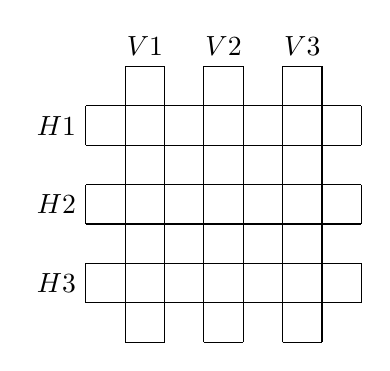
\begin{tikzpicture}[align=center]
\draw [scale=0.5,xshift=0cm, yshift=0cm] (0, 0) grid (1, 7) node [below] at (0.5cm,8cm) {$V1$};
\draw [scale=0.5,xshift=2cm, yshift=0cm] (0, 0) grid (1, 7) node [below] at (0.5cm,8cm) {$V2$};
\draw [scale=0.5,xshift=4cm, yshift=0cm] (0, 0) grid (1, 7) node [below] at (0.5cm,8cm) {$V3$};
\draw [scale=0.5,xshift=-1cm,yshift=5cm] (0, 0) grid (7, 1) node [left] at (0cm,0.5cm) {$H1$};
\draw [scale=0.5,xshift=-1cm,yshift=3cm] (0, 0) grid (7, 1) node [left] at (0cm,0.5cm) {$H2$};
\draw [scale=0.5,xshift=-1cm,yshift=1cm] (0, 0) grid (7, 1) node [left] at (0cm,0.5cm) {$H3$};
\end{tikzpicture}
\end{latin}

پایگاه داده زیر یک فرهنگ لغت شامل کلمات بالاست:

\begin{latin}
\begin{lstlisting}
word(abalone,a,b,a,l,o,n,e).
word(abandon,a,b,a,n,d,o,n).
word(enhance,e,n,h,a,n,c,e).
word(anagram,a,n,a,g,r,a,m).
word(connect,c,o,n,n,e,c,t).
word(elegant,e,l,e,g,a,n,t).
\end{lstlisting}
\end{latin}

محمول \متن‌لاتین{crosswd/6} را که نحوه پر کردن جدول با این لغات را تعریف می‌کند، بنویسید بطوری که سه آرگومان اول کلماتی باشند که ستون‌ها را از چپ به راست پر می‌کنند و سه آرگومان دوم کلماتی باشند که سطر ها را از بالا به پایین پر می‌کنند.

\end{exercise}

\clearpage

\section{تمرین عملی}

تاکنون کار با پرولوگ را فرا گرفته‌اید. در این قسمت می‌خواهیم اتحاد و اثبات جستجو را تمرین کنیم.

برای شروع برنامه پرولوگ خود را باز کنید تا خط فرمانی شبیه \متن‌لاتین{?-} را ببینید.

حالا پاسخ‌های خود به پرسش \verb!2.1! را تصحیح کنید. به این صورت که توسط محمول \متن‌لاتین{=/2} سعی کنید ترم‌های موجود در صورت سوال را متحد کنید. برای مثال، دو ترم \متن‌لاتین{food(bread,X)} و \متن‌لاتین{food(Y,sausage)} را امتحان می‌کنیم:

\begin{latin}
\begin{lstlisting}
?- food(bread,X) = food(Y,sausage).
X = sausage, Y = bread.
\end{lstlisting}
\end{latin}

همچنین ببینید چه اتفاقی می‌افتد اگر سعی کنید ترم‌هایی به شکل زیر را با هم متحد کنید:

\begin{latin}
\begin{lstlisting}
g(X,Y) = Y.
\end{lstlisting}
\end{latin}

وقت آن است که با یک محمول جدید از قبل تعریف شده در پرولوگ آشنا شویم، محمول  \verb!\=/2!. این محمول عکس محمول \متن‌لاتین{=/2} کار می‌کند: هنگامی پاسخ درست است که دو آرگومان آن متحد نشوند. مثلاً برای دو ترم a و b داریم:

\begin{latin}
\begin{lstlisting}
?- a \= b.
true.
\end{lstlisting}
\end{latin}

سعی کنید با این محمول کار کنید و مثال‌های زیر را امتحان کنید. البته اینکار را بدین صورت انجام دهید که ابتدا فکر کنید پرولوگ چه پاسخی خواهد داد، سپس ترم‌ها را وارد کنید تا ببینید پاسخ ذهنی شما درست بوده‌است یا خیر.

\begin{latin}
\begin{enumerate}
\item \verb!a \= a!
\item \verb!'a' \= a!
\item \verb!A \= a!
\item \verb!f(a) \= a!
\item \verb!f(a) \= A!
\item \verb!f(A) \= f(a)!
\item \verb!g(a,B,c) \= g(A,b,C)!
\item \verb!g(a,b,c) \= g(A,C)!
\item \verb!f(X) \= X!
\end{enumerate}
\end{latin}

همانطور که متوجه شدید محمول \verb!\=/2!نقیض محمول \متن‌لاتین{=/2} است: یک query توسط \متن‌لاتین{=/2} ارضاء می‌شود هرگاه توسط \verb!\=/2! ارضاء‌ نشود.

حال می‌خواهیم با یک محمول از پیش تعریف شده دیگر به اسم trace آشنا شویم. این محمول پرولوگ را مجبور می‌سازد که پردازش query ها را مرحله به مرحله انجام دهد و در هر مرحله نحوه اجرا را گزارش دهد. با اجرای هر مرحله پرولوگ منتظر می‌ماند تا شما با فشار دادن کلید enter دستور ادامه را صادر کنید. این دستور به عنوان یک ابزار برای عیب‌یابی\پانوشت{debugging} بکار می‌رود اما می‌توان از آن برای یادگیری نحوه کار جتسجوی اثبات در پرولوگ هم استفاده کرد.

در این فصل دیدیم که جستجوی اثبات برای پرسش \متن‌لاتین{k(X)} با توجه به پایگاه داده زیر، چطور پیش می‌رود.

\begin{latin}
\begin{lstlisting}
f(a).
f(b).
g(a).
g(b).
h(b).
k(X) :- f(X),g(X),h(X).
\end{lstlisting}
\end{latin}

این پایگاه داده را در فایلی با نام \متن‌لاتین{proof.pl} قرار دهید و آن را در پرولوگ بارگزاری کنید.

\begin{latin}
\begin{lstlisting}
?- [proof].
% proof compiled 0.00 sec, 6 clauses.
true.
\end{lstlisting}
\end{latin}

حال محمول «\متن‌لاتین{trace.}» را تایپ کرده و کلید enter را فشار دهید.

\begin{latin}
\begin{lstlisting}
?- trace.
true.
[trace]  ?-
\end{lstlisting}
\end{latin}

حالا پرولوگ در مد trace قرار دارد و تمام query ها را مرحله به مرحله مانند توضیحات بالا اجرا می‌کند. پرسش \متن‌لاتین{k(X).} را تایپ کنید و دکمه enter را فشار دهید. هر بار که با یک علامت سوال روبرو شدید دکمه enter را فشار دهید. با اینکار چیزی شبیه خروجی زیر مشاهده خواهید کرد:

\begin{latin}
\begin{lstlisting}
[trace]  ?- k(X).
   Call: (6) k(_G1412) ? creep
   Call: (7) f(_G1412) ? creep
   Exit: (7) f(a) ? creep
   Call: (7) g(a) ? creep
   Exit: (7) g(a) ? creep
   Call: (7) h(a) ? creep
   Fail: (7) h(a) ? creep
   Redo: (7) f(_G1412) ? creep
   Exit: (7) f(b) ? creep
   Call: (7) g(b) ? creep
   Exit: (7) g(b) ? creep
   Call: (7) h(b) ? creep
   Exit: (7) h(b) ? creep
   Exit: (6) k(b) ? creep
X = b.
\end{lstlisting}
\end{latin}

این خروجی را بدقت بخوانید و سعی کنید ارتباط هر خط با نحوه کار جستجوی اثبات را دریابید. مثلاً در خط هشتم، Redo نشان‌دهنده backtrack است که در متن فصل به آن اشاره کردیم.

برای یادگیری پرولوگ از trace زیاد استفاده کنید. اینکار به شما کمک می‌کند تا با نحوه کار پرولوگ بیشتر آشنا شوید. هرگاه دیگر نخواستید از trace استفاده کنید، دستور notrace را تایپ کنید تا پرولوگ از این حالت خارج شود:

\begin{latin}
\begin{lstlisting}
[trace]  ?- notrace.
true.
?-
\end{lstlisting}
\end{latin}